\documentclass{article}

\usepackage{amsmath} % math stuff
\usepackage{amssymb} % math stuff
\usepackage{array} % equations and stuff
\usepackage{bm} % bold math
%\usepackage{booktabs} % extra table rule options
%\usepackage{caption} % suppressed table numbering; incompatible with revtex, and longtable, I think
\usepackage{comment} % comment environment
%\usepackage{enumitem} % customization of enumeration, itemize, and description
\usepackage[T1]{fontenc} % font encoding for special characters, must also use scalable font package
\usepackage[margin=0.8in]{geometry} % paper sizes and margins (but be careful not to mess up pre-defined pages)
\usepackage{graphicx} % for graphics
%\usepackage{helvet} % default font is the helvetica postscript font
\usepackage[utf8]{inputenc} % special characters in tex input
\usepackage{layouts} % print units like widths
\usepackage{lipsum} % lorem ipsum filler text
\usepackage{lmodern} % scalable font?
\usepackage{longtable} % multi-page tables
\usepackage{makecell} % specify line-breaks in table cells
\usepackage{mathrsfs} % math script font
\usepackage{mhchem} % easier chemical formula
\usepackage{microtype} % allows disabling of ligatures
\usepackage{multicol} % multicolumns
%\usepackage{newcent} % new century schoolbook font
\usepackage{nicefrac}
\usepackage{numprint} % print and format (large) numbers
\usepackage{parskip} % removes paragraph indentation, and adjusts paragraph skip, as well as list items
\usepackage{pdfpages} % add pdf files as pages
%\usepackage{setspace} % adjust text spacing and indents
\usepackage{siunitx} % decimal alignment
\usepackage{subfigure} % divided figures
%\usepackage{tabu} % extra table options
\usepackage{textcomp} % symbols
\usepackage{threeparttablex} % better footnotes with longtable
\usepackage{titling} % title placement
\usepackage{ulem} % strikethrough text
%\usepackage{url} % superceded by hyperref
\usepackage{verbatim} % verbatim environment
\usepackage{xcolor} % colors and color boxes
\usepackage{xspace} % commands that don't eat up white space
\usepackage{hyperref} % links and page setup; should always come last

\hypersetup{
 bookmarks=true,
 colorlinks=true,
 citecolor=blue,
 linkcolor=blue,
 urlcolor=blue,
 pdfstartview={XYZ null null 1.0} % default open view is 100%
}

\DisableLigatures[f,t]{encoding = T1} % disable ff, fi, fl, tt ligatures; without options, it also disables -- = endash
\renewcommand{\arraystretch}{1.0} % extra vertical (and horizontal?) space in tables

% define centered, left- and right-aligned columns with specified widths
\newcommand{\PreserveBackslash}[1]{\let\temp=\\#1\let\\=\temp}
\newcolumntype{C}[1]{>{\PreserveBackslash\centering}p{#1}}
\newcolumntype{L}[1]{>{\PreserveBackslash\raggedright}p{#1}}
\newcolumntype{R}[1]{>{\PreserveBackslash\raggedleft}p{#1}}

\begin{document}

\pagestyle{empty} % don't number pages

% custom title
\begin{center}
{\LARGE Classic Riddler}

\vspace{0.15in}

{\Large 18 June 2021}
\end{center}


\section*{Riddle:}

Eight two-way roads all converge at a single intersection, as shown in the diagram below.

\vspace{0.1in}
\begin{center}

\includegraphics[width=2in]{roads_1.png}
\end{center}
\vspace{0.1in}

Two cars are heading toward the single intersection from different directions chosen at random.
Upon reaching the intersection, they both turn in a random direction (where proceeding straight is a possible ``turn'')---however, neither car pulls a U-turn (i.e., heads back the way it came).

In some cases, the paths of the cars can be drawn so that they do not cross.
In this case, all is well.

\vspace{0.1in}
\begin{center}
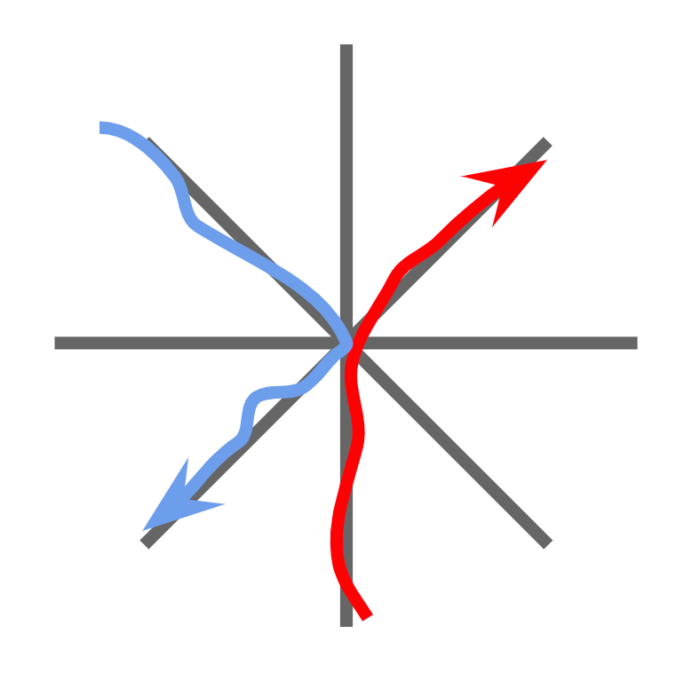
\includegraphics[width=2in]{roads_2.png}
\end{center}
\vspace{0.1in}

However, in other cases, the paths \textit{must} cross.
In this event, the cars will crash.

\vspace{0.1in}
\begin{center}
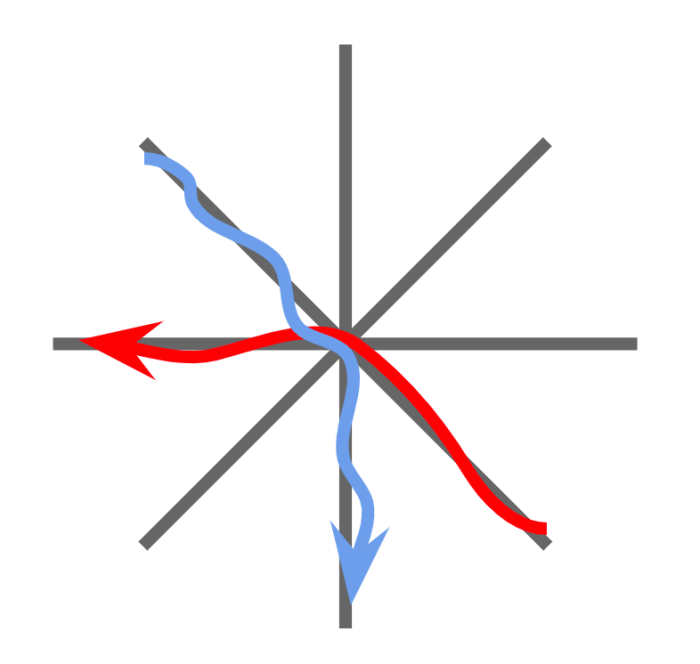
\includegraphics[width=2in]{roads_3.png}
\end{center}
\vspace{0.1in}

What is the probability the cars will crash?
(If both cars head off in the same direction, that also counts as a crash.)

\textit{Extra credit}: As the number of two-way roads converging at the intersection approaches infinity, what value does the probability of crashing approach?



\section*{Solution:}

For my discussion of the solution, I will arbitrarily label each of the roads A--H, as shown below:

\vspace{0.1in}
\begin{center}
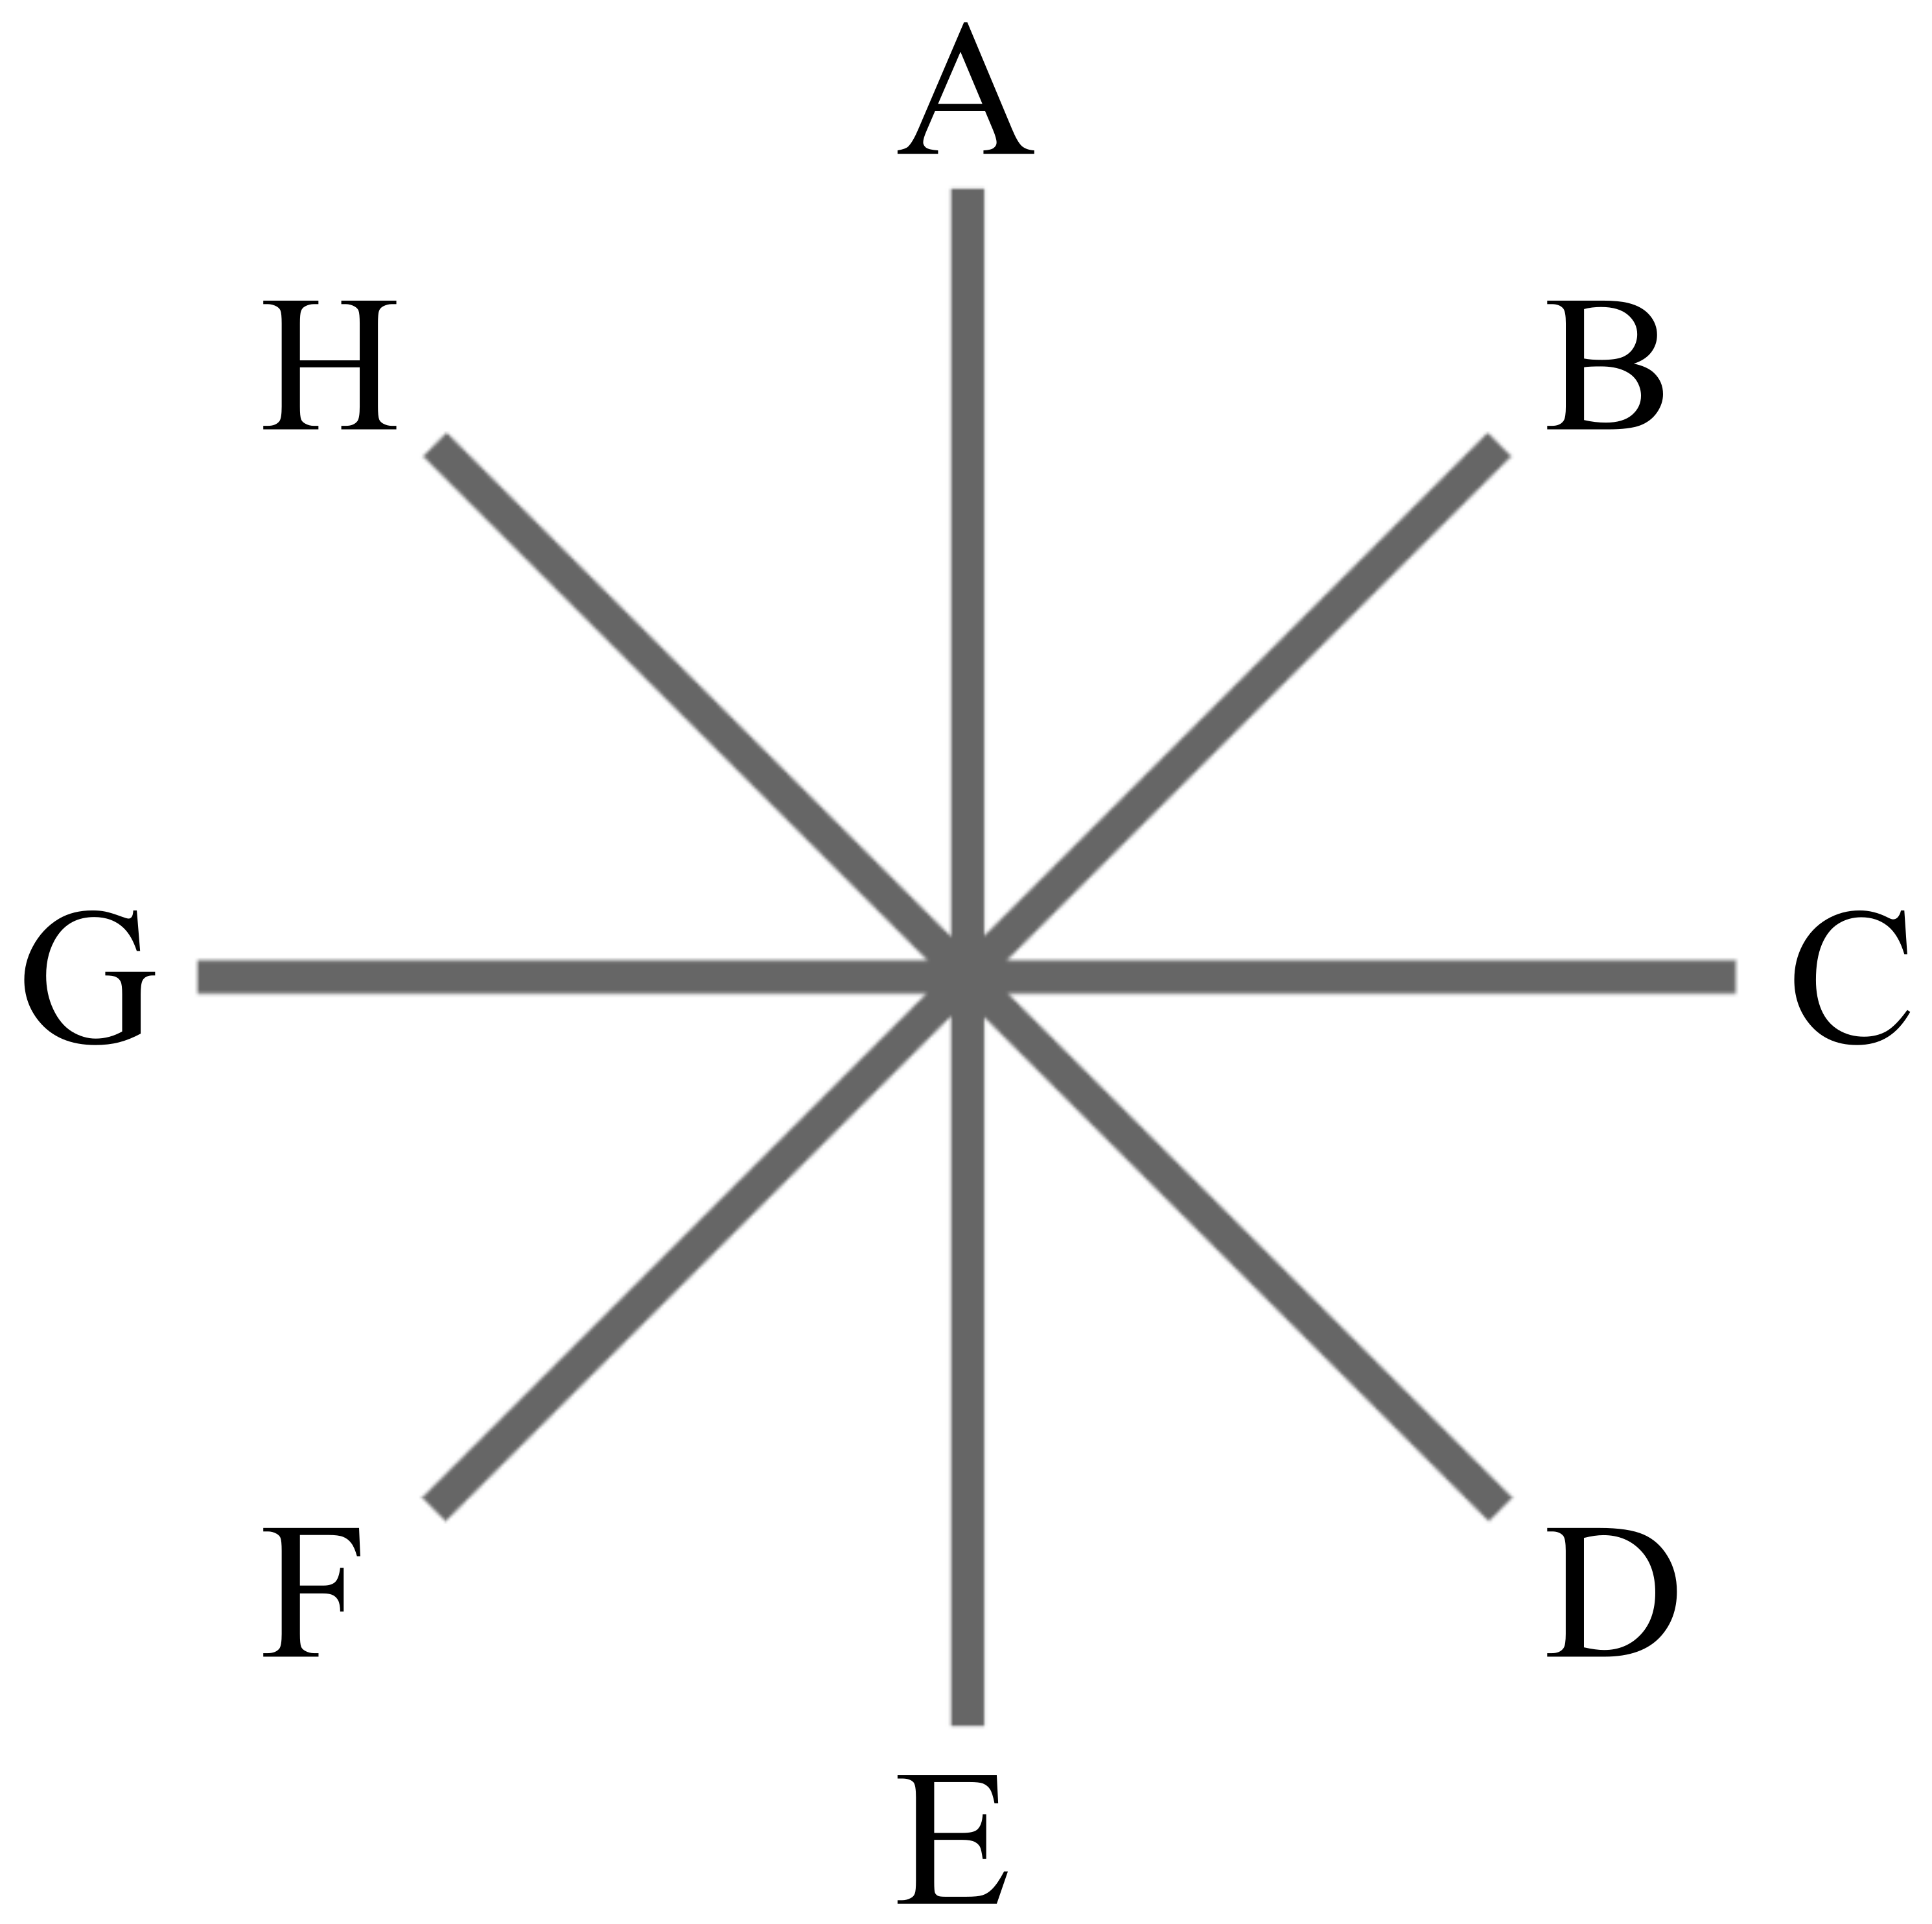
\includegraphics[width=2in]{roads_labeled.png}
\end{center}
\vspace{0.1in}

Without loss of generality, I will assume that one driver (say, red) always enters from road A.
Then, there are seven ways for A to exit.
The other driver must enter from any of the other seven roads and also has seven ways to leave.
That gives a total of $7^{3}=343$ scenarios to consider.
For my solution, I assume that a crash occurs when either 1) both cars exit through the same road, or 2) at least one car exits where the other car enters.

I listed out on paper all the ways for the two cars to crash, sorted by the entrances.
For example, if the cars enter in A and B, there are 34 ways to crash (out of 49 possibilities).
Specifically, if the first car exits through B (I will label this [AB][B?]), there is a crash no matter where the other car exits (seven crashes).
Similarly, for [AC][B?], there are seven crashes.
For [AD][B?], only [AD][BC] avoids a crash, leaving six other crashes.
For [AE][B?], there are five crashes; for [AF][B?], there are four crashes; for [AG][B?], there are three crashes; for [Ah][B?], there are two crashes.

With my assumptions, the calculation for [A?][H?] is the same as [A?][B?], also with 34 crashes out of 49 possibilities.
For [A?][C?] and [A?][G?], there are 29 ways to crash; for [A?][D?] and [A?][F?], there are 26 ways to crash; for [A?][G?], there are 25 ways to crash.
This gives a total of 203 crashes.
So the solution is
\fcolorbox{red}{white}{$\bm{{\nicefrac{203}{343}\approx0.592}}$}\,.

Another way to approach the problem is to assume that the roads have directional lanes (and of course, that the drivers stay in their lanes and make proper turns).
With this assumption, there are fewer crashes.
For example, the [AB][BA] scenario no longer results in a crash.
With this assumption, the probability of a crash is reduced to
\fcolorbox{red}{white}{$\bm{{\nicefrac{154}{343}\approx0.449}}$}\,.
It is worth noting that this answer does not depend on which side cars are driven; each situation is just a mirror of the other.

The extra credit is essentially asking what happens as the number of roads approaches infinity.
In this limit, the cars will never exit on the same road, nor will either car exit where the other entered.
So a crash only occurs if their paths cross, in a proper sense.
The question then becomes how many ways are there to connect four points on a circle (two entrances and two exits) with two lines such that the lines cross.
There are three total ways to connect the points, and in only one way do the lines cross.
If the points are labeled A, B, C, and D around the circle, then [AB][CD] and [AD][BC] do not have crossing lines, while [AC][BD] does have crossing lines.
Therefore, the solution to the extra credit is
\fcolorbox{red}{white}{\bf\nicefrac{1}{3}}\,.





\end{document}